% Since writing this up, it was decided to leave as future work. Still, worth
% having around for editing into such future work.

\documentclass[]{article}
\begin{document}

\title{Interestingness Measures for Theory Exploration}

\author{Chris Warburton}

\affil{University of Dundee,\\
\texttt{http://tocai.computing.dundee.ac.uk}}

\maketitle              % typeset the title of the contribution

\begin{abstract}
Since their inception, computers have been applied to automate and assist work in mathematics, with established fields including numerical computation, computer algebra, (online) communication and so on. Here we focus on their use in two areas: formal proof and statistics; and how new approaches are bringing these seemingly disparate disciplines closer together.
\end{abstract}

\section{Introduction}

As computers and software become more capable, and as our reliance on them increases, the importance of \emph{understanding}, \emph{predicting} and \emph{verifying} these systems grows; which is undermined by their ever-increasing complexity. Mathematics provides us with powerful, systematic methods of reasoning, which we can bring to bear on this challenge; in particular those of \emph{formal logic} and \emph{statistics}. By (partially) mechanising these approaches, in the fields of \emph{theorem proving} and \emph{machine learning}, respectively, we can leverage these increasing machine capabilities and direct them for the purpose of analysis. However, the question still remains: on what should we focus that analysis?

In this work, we investigate the notion of \emph{interestingness} in the exploration of formal systems (an area known as \emph{theory exploration}) as a way to make productive use of resources in an often intractable domain. To keep things concrete, we focus our formal analysis on equational formulae describing programs in the Haskell language, for reasons elaborated in \S \ref{sec:haskell}. Conceptually, we maintain a broader view, and survey many related areas which may offer insights on the problem.

Appeals to interestingness arise when more direct measures, such as utility, are not available. For example, the inclusion of particular statements in a program or proof development can be easily justified based on their contribution to the overall solution; however, in a \emph{library} there is no particular problem being solved, in which case we must judge statements on less direct criteria, such as how ``interesting'' they may be to our users. Appeals to interestingness abound in the history of computer-assisted reasoning; for example, in 1971 Plotkin \cite{plotkin1971further} considered the task of \textquote{discovering theorems $T$ from a system of axioms $Ax$}, and in particular the questions \textquote{Under what conditions is $T$ an interesting, possible theorem in the system $Ax$?} and \textquote{Is there a way to generate (most) interesting possible theorems?}. Despite such widespread use of the term, there is no standard definition of what makes a formal object, whether it is an axiom, a conjecture, a proof, etc., ``interesting''; although many ad-hoc heuristics have been proposed.

We begin our undertaking in \S \ref{sec:background} by introducing the Haskell language, as well as the relevant fields of verification for context. We define a formal framework for our investigation, and show how it relates to the existing theorem proving landscape. A selection of theorem proving scenarios which \emph{require} exploration are discussed in \S \ref{sec:examples}, whilst related work, including existing defintions of interestingness, is surveyed in \S \ref{sec:related}. We also review the use of exploration in other fields of Artificial Intelligence and Machine Learning, where researchers are experimenting with replacing \emph{explicit} goals and rewards with \emph{implicit} alternatives such as interestingness. Recent efforts in this area have lead to the emergence of principled theories, mostly based around (algorithmic) information theory, which may be adapted to our theory exploration context.

We discuss our present contributions in \S \ref{sec:current} and future research directions in \S \ref{sec:future}, before concluding in \S \ref{sec:conclusion}.

\begin{description}
\item{Interestingness}
  Various alternative interestingness criteria have been proposed, which we survey in \S \ref{sec:relatedwork}. Augmenting or replacing the criteria may be useful, for example to distinguish useful relationships from incidental coincidences; or to prevent surprising, insightful equations from being discarded because they can be simplified.
\end{description}

% Theory exploration is similar to \emph{experimental mathematics}

% - Relation to Science
%  - Testable/falsifiable hypotheses are like evaluable terms (or, more generally, conjectures which can be decided, using a reasonable amount of resources).
% - Relation to AI tasks: exploring surroundings, etc.

% - Statistics is another area that's less straightforward than normal numerical computing, since there is subjectivity and judgement involved in the answering of questions.

% Theory formation: Alison? Others.
% Theory exploration: Buchberger, Moa in Isabelle, Koen in Haskell. Others?
% Theorem proving: Well-trodden: first-order ATP, higher-order ITP, functional programming
% Communication: Latex, Wikis, APIs, communicating with aliens

\section{Exploration in Theorem Proving}
\label{sec:examples}

Before exploring abstract definitions of interestingness, we can first consider some scenarios which arise during formal proof where we are forced to generate conjectures. An analysis of these situations, and the subsequent theorems they produce, will contribute towards an empirical justification for what is interesting (at least from a utilitarian point of view) and inform our later exploration of the literature.

\subsection{Generalisation}

\providecommand{\coq}[1]{\lstinline[language=ML]|#1|}

When we \emph{generalise} a statement $S$, we obtain a new statement $S'$ of which $S$ is a special case. Although it seems counterintuitive, a generalised statement can sometimes be \emph{easier} to prove than the original. This arises often in inductive proofs, since the specific obligations which arise in the proof may be incompatible with the available inductive hypotheses.

However, we cannot blindly generalise \emph{all} obligations we encounter, since \emph{over-generalising} results in obligations which are so strong that they are unprovable, or even false. We must therefore rely on heuristics to guide the generation of generalised conjectures, and hence perform a kind of exploration.

An informative example is given by Boyer and Moore of the associativity of multiplication in ACL2 \cite{boyer1983proof}:

$$(x * y) * z = x * (y * z)$$

During the course of the proof, the following obligation arises:

\begin{equation}
  \tag{conc3}
  (y + (x * y)) * z = (y * z) + ((x * y) * z)
  \label{eq:conc3}
\end{equation}

ACL2 automatically generalises \eqref{eq:conc3} by replacing the repeated sub-term $x * y$ with a fresh variable $w$:

\begin{equation}
  \tag{conc4}
  (y + w) * z = (y * z) + (w * z)
  \label{eq:conc4}
\end{equation}

This generalised form is clearly the distributivity law for multiplication and addition, which can be proved separately to the original goal of associativity. It would not be controversial to claim that this distributivity law is interesting in its own right (relative to associativity, at least), in addition to its usefulness in making this proof go through.

% TODO: Describe the ACL2 heuristics

Generalisation also occurs frequently when reasoning about \emph{tail-recursive} definitions \cite{kapur2003automatic}. \footnote{A tail-recursive function can be executed in constant space using a loop, whereas recursion in non-tail positions may require a growing number of stack frames or nested closures. See \S \ref{sec:auxiliarylemmas} for example definitions of each type.}

\subsection{Analogy}

One way to characterise the interestingness of a statement is by \emph{analogy} to existing interesting statements. By finding lemmas analogous to those of a different theory, we may be able to re-use tactics and other forms of meta-programming across both.

Existing theory exploration systems have been successfully applied to this problem, however the use of pure exploration misses opportunities to \emph{focus} the search, since we know which lemmas are used in those theories where a technique succeeded. If we can find an analogy to map from such solved problems to our unsolved goal, we can infer the approximate form of the lemmas we require, and target these specifically.

The approach taken by \textsc{ACL2(ml)} is to find lemmas which may be relevant to solving a goal $G$ by making analogies via unsupervised clustering \cite{Heras.Komendantskaya.Johansson.ea:2013}. These clusters are used in two ways:

\begin{itemize}

  \item First, we use the cluster $C_G$ containing $G$ to identify analogous theorems.

  \item For each theorem $T \in C_G \setminus \{G\}$, we consider those symbols $S_T$ which occur in $T$ but not in $G$. Our analogous lemmas are those used to prove $T$, mutated such that symbols $s \in S_T$ are replaced by members of the cluster $C_s$ containing $s$.

\end{itemize}

The running examples for demonstrating \textsc{ACL2(ml)} are equivalence theorems for tail-recursive and non-tail-recursive calculations, as well as the effect of repeating certain list operations:

\begin{itemize}

  \item $\forall n, \texttt{natp}(n) \rightarrow \texttt{fact-tail}(n) = \texttt{fact}(n)$ where \texttt{natp} is the predicate that $n$ is a natural number, whilst \texttt{fact-tail} and \texttt{fact} are tail-recursive and non-tail-recursive implementations of factorial, respectively.

  \item $\forall n, \texttt{natp}(n) \rightarrow \texttt{power-tail}(n) = \texttt{power}(n)$,  where \texttt{power-tail} and \texttt{power} calculate powers of 2.

  \item $\forall n, \texttt{natp}(n) \rightarrow \texttt{fib-tail}(n) = \texttt{fib}(n)$,  where \texttt{fib-tail} and \texttt{fib} calculate fibonacci numbers.

  \item $\forall x, \texttt{nat-listp}(x) \rightarrow \texttt{sort}(\texttt{sort}(x)) = \texttt{sort}(x)$, for list-of-natural-numbers predicate \texttt{nat-listp} and list-sorting function \texttt{sort}.

  \item $\forall x, \texttt{true-listp}(x) \rightarrow \texttt{rev}(\texttt{rev}(x)) = x$, where \texttt{true-listp} ensures that $x$ is a valid singly-linked list structure and \texttt{rev} is list reversal.

  \item $\forall x, \texttt{true-listp}(x) \rightarrow \texttt{int}(x, x) = x$, where \texttt{int} is the intersection of lists (i.e. a list of elements common to each).

\end{itemize}

\subsection{Auxiliary Lemmas} \label{sec:auxiliarylemmas}

One consideration when generating conjectures is the difference between theorems, lemmas, corollaries, etc. From a logical point of view, these are all equivalent, and hence most proof assistants do not distinguish between them. However, their \emph{intention} may be different: in a sense, theorems are the interesting results; whilst lemmas are useful results, required for proving the theorems.

Some systems, like Coq, allow users to \emph{label} each statement as being a \coq{Theorem}, a \coq{Lemma}, etc. despite their internal representations being the same. This shows us immediately that lemmas outnumber theorems; in the Coq standard library there are over five times as many lemmas as theorems \footnote{The latest version as of writing is \texttt{coq-8.4pl6} which, when excluding comments, includes 1492 occurences of \coq{Theorem} and 7594 of \coq{Lemma} in its \texttt{theories/} directory.}.

% TODO: Analyse them

% TODO: Theory exploration as lemma generation; give example from a HipSpec paper

We can find a need for auxiliary lemmas, once again, in the context of tail-recursive functions. Consider proving the (pointwise) equality of the following Coq functions, defined for the Peano naturals \coq{Z} and \coq{S}:

\begin{lstlisting}[language=ML, xleftmargin=.2\textwidth, xrightmargin=.2\textwidth]
Inductive Nat : Set := Z : Nat
                     | S : Nat -> Nat.

Fixpoint plus      (n m : Nat) := match n with
                                      | Z    => m
                                      | S n' => S (plus n' m)
                                  end.

Fixpoint plus_tail (n m : Nat) := match n with
                                      | Z    => m
                                      | S n' => plus_tail n' (S m)
                                  end.
\end{lstlisting}

\iffalse
Haskell equivalent:

plus :: Nat -> Nat -> Nat
plus      n  Z    = n
plus      n (S m) = S (plus n m)

plus_tail :: Nat -> Nat -> Nat
plus_tail n  Z    = n
plus_tail n (S m) = plus_tail (S n) m
\fi

Both of these functions implement addition, but the \coq{plus_tail} variant is tail-recursive. However, if we want to \emph{prove} that the definitions are (pointwise) equal, we run into difficulties. In particular, when the inductive step requires us to prove \coq{plus (S n) m = plus n (S m)} (which seems reasonable), we cannot make this go through using another inductive argument.

\iffalse

\begin{lstlisting}[language=ML, xleftmargin=.2\textwidth, xrightmargin=.2\textwidth]
(* Solve equalities by beta-normalising both sides *)
Ltac triv := try (simpl; reflexivity).

(* Prove equivalence of plus and plus_tail *)
Theorem equiv : forall n m, plus n m = plus_tail n m.
  induction n; triv. (* Base case is trivial *)

  (* Inductive case: plus (S n) m = plus_tail (S n) m *)
  intro m.

  (* Beta-reduce the right-hand-side (justification is trivial) *)
  replace (plus_tail (S n) m) with (plus_tail n (S m)); triv.

  (* Use induction hypothesis to replace plus_tail with plus *)
  rewrite <- (IHn (S m)).
\end{lstlisting}

\fi

Specifically, the \emph{conclusion} of a second inductive hypothesis is exactly the equation we need:

\begin{lstlisting}[language=ML, xleftmargin=.2\textwidth, xrightmargin=.2\textwidth]
IHn' : (forall x, plus n' x = plus_tail n' x) -> plus (S n') m = plus n' (S m)
\end{lstlisting}

Yet we cannot provide it with the argument it needs, as our original induction hypothesis is \emph{too specific} (i.e. it has too many \coq{S} constructors):

\begin{lstlisting}[language=ML, xleftmargin=.2\textwidth, xrightmargin=.2\textwidth]
IHn : forall x, plus (S n') x = plus_tail (S n') x
\end{lstlisting}

We are forced to abandon the proof, despite such a reasonable-looking intermediate goal.

In fact, if we attempt to prove that goal \emph{separately}, we can use a straightforward argument by induction; even though it is actually \emph{stronger} due to the absence of the \coq{IHn} assumption. Using this separate result as a lemma, the pointwise equality is proven easily.

\iffalse

\begin{lstlisting}[language=ML, xleftmargin=.2\textwidth, xrightmargin=.2\textwidth]
Lemma gen n m : plus (S n) m = plus n (S m).
  induction n; triv. (* Base case is trivial *)

  (* Move all S constructors outside *)
  simpl. rewrite <- IHn. simpl.

  (* Trivial *)
  reflexivity.
Defined.
\end{lstlisting}

\begin{lstlisting}[language=ML, xleftmargin=.2\textwidth, xrightmargin=.2\textwidth]
  rewrite (gen n m).
  reflexivity.
Defined.
\end{lstlisting}

\fi

\subsection{Tests} \label{sec:tests}

Since we are working in the domain of Haskell programs, an abundant source of statements are available in the form of \emph{tests}. For manually-written tests, the effort required to write them implies that they must be of some interest to their author. Many forms of test are \emph{not} suitable for our purposes, such as \emph{unit tests} which are always trivially provable by $\beta$-reduction; or \emph{integration tests}, which depend on the behaviour of the external environment. One reason to study Haskell is its widespread use of \emph{property checking}, which does give us useful data. Many Haskell property checkers exist, based on random testing (\textsc{QuickCheck} \cite{claessen2011quickcheck} and \textsc{SmartCheck} \cite{pike2014smartcheck}), enumeration (\textsc{SmallCheck} \cite{runciman2008smallcheck}), observation (\textsc{Lazy SmallCheck} \cite{reich2013advances}) and logic programming (\textsc{SparseCheck} \cite{sparsecheck}).

Thankfully the major differences between these systems are in the way they instantiate test arguments; their representations of properties are largely the same (modulo renaming of functions and types).

Here we consider the 10 most-downloaded packages from \textsc{Hackage} (as of 2015-10-30) which have property tests; these are \texttt{warp}, \texttt{aeson}, \texttt{text}, \texttt{lens}, \texttt{conduit}, \texttt{pandoc}, \texttt{attoparsec}, \texttt{scientific}, \texttt{yesod-core} and \texttt{blaze-html}.

% TODO: Analysis

\section{Related Work}
\label{sec:related}

\iffalse

\subsection{Conjecture Generation}

The task of \emph{conjecture generation} lies at the heart of theory exploration, and

\subsubsection{Lemma generation}

\fi

\subsection{Exploration in Artificial Intelligence}

Theorem proving is not the only area of AI to have automation extended from problem \emph{solving} to problem \emph{invention}. Here we consider similar approaches in a variety of domains, and identify techniques which could be re-purposed in the context of theory exploration.

\subsubsection{Evolutionary Computation}

\emph{Evolutionary computation} is an umbrella term for heuristic search algorithms which mimic the process of evolution by natural selection among a population of candidate solutions \cite{back1997evolutionary}. Whilst \emph{genetic algorithms} are perhaps the most well-known instance of evolutionary computation, their use of \emph{strings} to represent solutions causes complications when comparing to a domain like theory exploration, where recursive structures of unbounded depth arise. Thankfully these problems are not insurmountable, for example \emph{genetic programming} can operate on tree-structures natively \cite{banzhaf1998genetic}, which makes evolutionary computation a useful source of ideas for reuse in our theory exploration setting.

Traditionally, evolutionary approaches assign solutions a \emph{fitness} value, using a user-supplied \emph{fitness function}. Fitness should correlate with how well a solution solves the user's problem; for example, the fitness of a solution to some engineering problem may depend on the estimated materials cost. If we frame the task of theory exploration in evolutionary computation terms, the fitness function would be our interestingness measure.

Pure exploration (i.e. for its own sake) has been studied in evolutionary computation for two main reasons: \emph{artificial life} and \emph{deceptive problems}. The former attempts to gain insight into the nature of life and biology through competition over limited resources. Whilst this may have utility in resource allocation, e.g. efficient scheduling of a portfolio of ATP programs, there is no direct connection to interestingness in theory exploration, so we will not consider it further (note that similar resource-usage ideas can also be found in the literature on \emph{artificial economies}, e.g. \cite{baum2000evolution}).

On the other hand, work on deceptive problems is highly relevant, as it has lead to studying various notions of intrinsic fitness, which are analogous to the interestingness measures we want. Deceptive problems are those where \textquote{pursuing the objective may prevent the objective from being reached} \cite{lehman2011abandoning}, which is caused by the fitness (objective) function having many local optima which are easy to find (e.g. by hill climbing), but few global optima which are hard to find. Many approaches try to avoid deception by augmenting the given fitness function to promote \emph{diversity} and \emph{novelty}, such as \emph{niching methods} \cite{sareni1998fitness}.

One example is \emph{fitness sharing}, which divides up fitness values between identical or similar solutions. Say we have a user-provided fitness function $f$, and a population containing two identical solutions $s_1$ and $s_2$; hence $f(s_1) = f(s_2)$. In a fitness sharing scheme, we interpret fitness as a fixed resource, distributed according to $f$; when multiple individuals occupy the same point in the solution space, they must \emph{share} the fitness available there. We can describe the fitness \emph{allocated} to a solution by augmenting $f$, e.g. if we allocate fitness uniformly between identical solutions we get:

$$f'(x) = \frac{f(x)}{\sum_{i=1}^n \delta_{s_i x}}$$

Where $n$ is the population size, $s_i$ is the $i$th solution in the population and $\delta$ is the Kronecker delta function. In the example above, assuming there are no other copies in the population, then $f'(s_1) = \frac{f(s_1)}{2} = \frac{f(s_2)}{2} = f'(s_2)$. By sharing in this way, the fitness of each solution is balanced against redundancy in the population: there may still be many copies of a solution, but only when the fitness is high enough to justify all of them.

There are many variations on this theme, such as sharing between ``close'' solutions rather than just identical ones and judging distance based on fitness (AKA phenotypically) rather than based on the location in solution space (AKA genetically). Yet the underlying principle is always the same: penalise duplication in order to promote diversity. This lesson can be carried over to our theory exploration context, where a theorem should be considered less interesting if it is ``close'' to others which have been found.

In a similar way, we can bias our search procedure, rather than our fitness function, towards diversity. The search procedure in population-based evolutionary algorithms consists of \emph{selecting} one or more individuals from the population, e.g. via truncation (select the best $n$ individuals, discarding the rest); then \emph{transforming} the selected individuals, e.g. via mutation and crossover, to obtain new solutions.

\newcommand{\argmin}{\operatornamewithlimits{argmin}}

Traditional selection methods are biased towards high fitness individuals (this is especially clear for truncation). Alternative schemes have been proposed which favour diversity \emph{at the expense of} fitness. For example, the fitness uniform selection scheme (FUSS) \cite{hutter2002fitness} selects a target fitness $f_t$ uniformly from the interval $\left[ f_{min}, f_{max} \right]$ between the highest and lowest of the population. An individual $s$ is then selected with fitness closest to $f_t$, i.e. $s = \operatornamewithlimits{argmin}\limits_{x} \lvert f(x) - f_t \rvert$

In this way, the fitness function $f$ is used to assign comparable quantities to solutions, but it is not treated as the objective; instead, the implicit objective is to maintain a diverse population, with individuals spread out uniformly in fitness space. This approach seems useful for informing our work in theory exploration, as it supports search criteria which \emph{describe} solutions, but which we may not want to \emph{optimise}. As a simple example, we might distinguish different forms of theorem by measuring how balanced their syntax trees are (-1 for left-leaning, +1 for right leaning, 0 for balanced); but it would be senseless to \emph{maximise} how far they lean.

Once we begin this process of augmenting fitness functions, or abandoning their use as objectives, an obvious question arises: what happens if our new function contains nothing of the original? This kind of pure exploration scenario leads to a variety of ideas for \emph{instrinsic} fitness, such as novelty \cite{lehman2011abandoning}, which can lead to learning useful ``stepping stones'' even in objective-driven domains. Such intrinsic notions of fitness are direct analogues of the interestingness measures we seek for theory exploration.

\subsubsection{Artificial Curiosity}
\label{sec:curiosity}

\begin{figure}
  \centering
  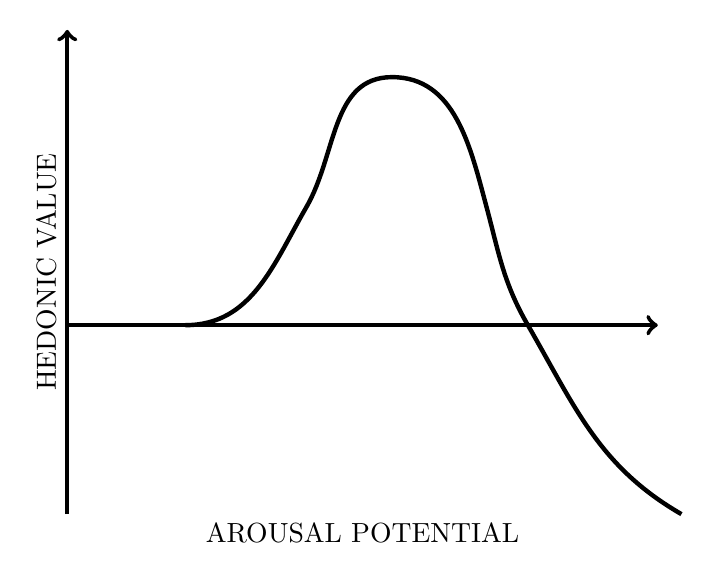
\begin{tikzpicture}[scale=0.75]
      % The image, for reference
      % \node[anchor=south west,inner sep=0] at (0,0) {\includegraphics[width=\textwidth]{wundt.png}};

      % Axes
      \draw[black,ultra thick,->] (1,0.8) -- (1,  9)   node[midway, above, sloped] {HEDONIC VALUE};     % y axis
      \draw[black,ultra thick,->] (1,4)   -- (11, 4);                                                   % x axis
      \path                       (1,0.8) -- (11, 0.8) node[midway, below]         {AROUSAL POTENTIAL}; % x axis label

      % Curve. The numbers come from tracing over wundt.png
      \draw[black,ultra thick] (3, 4)
           to[out=0,   in=240] (5.05, 6)
           to[out=60,  in=180] (6.5,  8.2)
           to[out=0,   in=105] (8.1,  6)
           to[out=-75, in=120] (8.8,  4)
           to[out=-60, in=150] (11.4, 0.8);

      % This version is closer, but a little jagged
      \iffalse
      \draw[black,ultra thick] (3, 4)
           to[out=0,   in=240] (5.05, 6)
           to[out=60,  in=225] (6,    8)
           to[out=45,  in=180] (6.5,  8.2)
           to[out=0,   in=135] (7.2,  8)
           to[out=-45, in=105] (8.1,  6)
           to[out=-75, in=120] (8.8,  4)
           to[out=-60, in=150] (11.4, 0.8);
      \fi
  \end{tikzpicture}

  \caption{The Wundt curve, reproduced from \cite{berlyne1970novelty}. The axes ``hedonic value'' and ``arousal potential'' are described as covering \textquote{reward value\dots preference or pleasure}, and \textquote{all the stimulus properties that tend to raise arousal, including novelty and complexity}, respectively.}

  \label{fig:wundt}
\end{figure}

\emph{Artificial curiosity} (AC) describes active learning systems which are rewarded based on how interesting the input or data they discover is \cite{schmidhuber2006developmental}. Although framed in the context of \emph{reinforcement learning}, this is clearly relevant to our theory exploration setting.

As an unsupervised learning task, AC has no access to labels or meanings associated with its input; the only features it can learn are the structure and relationships inherent in the data, which is very much what we would like a theory exploration system to do. The unifying principle of AC methods is to force systems away from inputs which are not amenable to learning; either because they are so familiar that there is nothing left to learn, or so unfamiliar that they are unintelligible. The resulting behaviour is characterised by the \emph{Wundt curve} (shown in figure \ref{fig:wundt}) \footnote{In practice, many measures avoid negative values for simplicity, in which cases we replace all negative points on the curve with zero.}, which has been used in psychology to explain human aesthetics and preferences \cite{berlyne1970novelty}.

We can divide AC approaches into two groups: the first, which we call \emph{explicit}, send inputs which follow a Wundt curve to their learning algorithm; the second, the \emph{implicit} approaches, instead modify the \emph{output} of their learning algorithm(s), such that the overall system follows a Wundt curve as an emergent property.

In the explicit case, the \emph{implicit reward} signals being learned are analogous to our notion of interestingness. A framework encompassing many examples is given in \cite{oudeyer2007intrinsic} in the context of reinforcement learning.

One particularly general measure is \emph{compression progress}: given a compressed representation of our previous observations, the ``progress'' is the space saved if we include the current observation. Observations which are incompressible or trivially compressible don't save any space, whilst observations which provide new information relevant to past experience can provide a saving. This can be translated to a theorem proving context very naturally: our observations are theorems and their proofs, whilst new theorems which generalise known results will allow us to compress their proofs.

% TODO: Examples
\cite{Schmidhuber1999}

Two sources of intrinsic reward are proposed in \cite{Hester.Stone:2012} for \emph{random forests}. A random forest is a population of decision trees, where each tree is trained on a sub-set of the available examples, each decision is made using a sub-set of the available features, and the predictions of every tree are averaged to obtain that of the forest \cite{randomforests}. The first intrinsic reward is the \emph{disagreement} between predictions; for a forest with $m$ models (trees), predicting features $x_1$ \dots $x_n$ of the state resulting from taking action $a$ in state $s$, we simply sum the Kullback-Leibler divergence $D_{\rm KL}$ of each prediction $P_1$ \dots $P_m$ from every other prediction:

\begin{equation}
  D(s,a) = \sum_{i = 1}^n \sum_{j = 1}^m \sum_{k = 1}^m D_{KL}(P_j(x_i|s,a) || P_k(x_i|s,a))
\end{equation}

$D(s,a)$ is an explicit AC reward, as it follows a Wundt curve as the complexity of transitions increases. For parts of the state space which have been fully learned, the models will agree on accurate predictions. For parts which are unlearnable, the models cannot infer any structure, and will converge to reporting the average of past observations; these predictions may not be accurate, but they will be in agreement. Hence it is the states which are amenable to learning which produce the largest disagreement.

The second intrinsic reward is simply a measure of distance from previous observations, which pushes the system towards unseen states regardless of how learnable they are (similar to the $R_{max}$ technique). This is too simple to meet our definition of AC, but it does force the models to generalise their predictions to unexplored states, acting to increase disagreement in the forest.

A key advantage of random forests is that their models are \emph{inspectable}: they not only give predictions, but also \emph{reasons} for those predictions (i.e. we can see which paths are taken through each decision tree). % TODO: The accuracy of these random forest models are compared

% TODO
\cite{Kaplan2006}
\cite{Lipson2007}
\cite{Luciw2011}
\cite{Macedo2000}
\cite{Ramik.Sabourin.Madani:2013}
\cite{Roa.Kruijff.Jacobsson:2009}
\cite{Schaul.Sun.Wierstra.ea:2011}
\cite{Schmidhuber1999}
\cite{Schmidhuber:1991}
\cite{Scott1989}
\cite{Steunebrink.Koutnik.Thorisson.ea:2013}
\cite{maher2008achieving}
\cite{meyer1991possibility}
\cite{oudeyer2004intelligent}
\cite{oudeyer2014evolution}
\cite{schmidhuber2006developmental}

% TODO: Coevolution

Whilst clearly of relevance to theory exploration, artificial curiosity is usually framed in the context of a \emph{reinforcement learning} and \emph{intrinsic reward}, especially in the field of developmental robotics. This requires non-trivial choices to be made in deciding which of its concepts are of relevance to our domain, and how they may be translated across. For example, much of developmental robotics studies continuous, real-valued sensorimotor signals which may not have any direct analogue in the manipulation of logical formulae. However, if we take a higher-level view, the study of such signals may provide insight for predicting and tuning the behaviour of off-the-shelf ATP algorithms.

The most obvious contrast between developmental robotics and theory exploration is that the latter is not physically embodied (e.g. in a robot). Embodiment has been proposed as a necessary property of intelligent systems, as it provides \emph{grounding} \cite{anderson2003embodied}. Embodiment emerged as a response to the symbolic techniques of GOFAI, and in this sense the fields of theory exploration and developmental robotics seem incompatible. Nevertheless, TE can be seen to avoid the problems of GOFAI in two ways:

\begin{itemize}

  \item Firstly, the abstract, mathematical domain being explored is not a \emph{model} of some external, physical environment; the domain \emph{is} our environment; hence there is no issue of grounding terms with some external meaning.

  \item Secondly, there is a physical aspect of TE in that \emph{resource usage} is a critical factor. If it weren't, then brute force enumeration of proofs would be a viable solution. In this sense, we can provide physical inputs to our algorithms, such as measures of time and space used.

\end{itemize}

\iffalse

\subsubsection{Universal Drives}

PhysRevLett.110.168702.pdf
Omohundro? Too physical.
\emph{Universal drives} are those

\fi

\subsection{Statistics of Formal Systems}

The core problem of assigning ``interestingness'' to logical formulae is the application of statistical reasoning to the discrete, semantically-rich domain of formal systems. This problem has been tackled from various directions for a variety of reasons; here we summarise those contributions which seem of particular importance for theory exploration.

\subsubsection{Relevance Filtering}
\label{sec:relevance}

% TODO
\cite{kuhlwein2012overview}

The combinatorial nature of formal systems causes many proof search methods, such as resolution, to have exponential complexity \cite{haken1985intractability}; hence even a modest size increase can turn a trivial problem into an intractable one. Finding efficient alternatives for such algorithms, especially those which are NP-complete (e.g. determining satisfiability) or co-NP-complete (e.g. determining tautologies), seems unlikely, as it would imply progress on the famously intractable open problems of $\text{P} = \text{NP}$ and $\text{NP} = \text{co-NP}$. On the other hand, we can turn this difficulty around: a modest \emph{decrease} in size may turn an intractable problem into a solvable one. We can ensure that the solutions to these reduced problems coincide with the original if we only remove \emph{redundant} information. This leads to the idea of \emph{relevance filtering}.

Relevance filtering simplifies a proof search problem by removing from consideration those clauses (axioms, definitions, lemmas, etc.) which are deemed \emph{irrelevant}. The technique is used in Sledgehammer during its translation of Isabelle/HOL theories to statements in first order logic: rather than translating the entire theory, only a sub-set of relevant clauses are included. This reduces the size of the problem and speeds up the proof search, but it creates the new problem of determining when a clause is relevant: how do we know what will be required, before we have the proof?

The initial approach, known as \textsc{MePO} (from \emph{Meng-Paulson} \cite{meng2009lightweight}), gives each clause a score based on the proportion $m / n$ of its symbols which are ``relevant'' (where $n$ is the number of symbols in the clause and $m$ is the number which are relevant). Initially, the relevant symbols are those which occur in the goal, but whenever a clause is found which scores more than a particular threshold, all of its symbols are then also considered relevant. There are other heuristics applied too, such as increasing the score of user-provided facts (e.g. given by keywords like \texttt{using}), locally-scoped facts, first-order facts and rarely-occuring facts. To choose $r$ relevant clauses for an ATP invocation, we simply order the clauses by decreasing score and take the first $r$ of them.

Recently, a variety of alternative algorithms have also been investigated, including:

\begin{description}

  \item{\textsc{MaSH}}: Machine Learning for SledgeHammer \cite{kuhlwein2013mash}. The distinguishing feature of \textsc{MaSH} is its use of ``visibility'', which is essentially a dependency graph of which theorems were used in the proofs of which other theorems; although theorems are represented as abstract sets of features. To select relevant clauses for a goal, the set of clauses which are visible from the goal's components is generated; this is further reduced by (an efficient approximation of) a naive Bayes algorithm.

  \item{\textsc{MOR}}: \emph{Multi-output ranking} uses a support vector machine (SVM) approach for selecting relevant axioms from the Mizar Mathematical Library for use by the Vampire ATP system \cite{alama2014premise}. \iffalse TODO: describe the kernel, as that's the interesting bit \fi It compares favourably to \textsc{SNoW} and \textsc{SInE}.

  % TODO:
  \item{\textsc{SInE}}
  \item{\textsc{BliStr}}
  \item{\textsc{HOLyHammer}}
  \item{\textsc{MoMM}}
  \item{\textsc{SNoW}}
  \item{\textsc{MPTP 0.2}}
  \item{\textsc{MaLARea}}
  \item{\textsc{MaLARea SG1}}

\end{description}

\subsubsection{Clustering}
\label{sec:clustering}

% TODO: ML4PG
\cite{journals/corr/abs-1212-3618}
% TODO: ACL2(ml) (also examples section)
\cite{heras2013proof}

\subsubsection{Probability of Sentences}

The most important property of a logical formula is its truth value. Although we may be able to determine some truth values exactly, e.g. using decision or semi-decision procedures, it may be more efficient to \emph{approximate} truth values. One straightforward extension of truth values is \emph{probabilities}, where we can assign probability $1$ to formulae which are known to be true, $0$ to formulae known to be false, and intermediate values to those which we do not yet know.

% TODO
\cite{Hutter.Lloyd.Ng.ea:2013}

\subsubsection{Interestingness in Concept Formation}
\label{sec:conceptformation}

% TODO:
\cite{Montano-Rivas.McCasland.Dixon.ea:2012}
\cite{Piantadosi.Tenenbaum.Goodman:2012}
\cite{Wille:2005}
\cite{colton1999automatic}
\cite{colton2000agent}
\cite{colton2012automated}
\cite{lenat1977automated}
\cite{mullerunderstanding}
\cite{Bundy.Cavallo.Dixon.ea:2015}
\cite{johansson2009isacosy}
\cite{spector2008genetic}
\cite{colton2012automated}
 \cite{geng2006interestingness}
% TODO: How does https en.wikipedia.org/wiki/Discovery system relate?

% However, this search space grows exponentially in the length of the proofs, which is unfortunate since proof length has been proposed as an approximate measure of how interesting a theorem is \cite[\S~10.2.1]{colton2012automated}.

% Alan Bundy et al

% Eurisko, AM, etc.?

\subsubsection{Learning From Structured Data}

One major difficulty with formal mathematics as a domain in which to apply statistical machine learning is the use of \emph{structure} to encode information in objects. In particular, \emph{trees} appear in many places: from inductive datatypes, to recursive function definitions; from theorem statements, to proof objects. Such nested structures may extend to arbitrary depth, which makes them difficult to represent with a fixed number of features, as is expected by most machine learning algorithms. Here we review a selection of solutions to this problem, and compare their distinguishing properties.

\paragraph{Feature Extraction}\label{sec:featureextraction}

\emph{Feature extraction} is a common pre-processing step for machine learning (ML). Rather than feeding ``raw'' data straight into our ML algorithm, we only learn a sample of \emph{relevant} details, known as \emph{features}. This has two benefits:

\begin{itemize}
  \item \emph{Feature vectors} (ordered sets of features) are chosen to be more compact than the data they're extracted from: feature extraction is \emph{lossy compression}. This reduces the size of the ML problem, improving efficiency (e.g. running time).
  \item We avoid learning irrelevant details such as the encoding system used, improving \emph{data} efficiency (the number of samples required to spot a pattern).
\end{itemize}

Another benefit of feature extraction is to \emph{normalise} the input data to a fixed-size representation. Many ML algorithms only work with fixed-size inputs; for example, the popular \emph{backpropagation} \cite{Russell:2003:AIM:773294} algorithm works on models with \emph{fixed} topology (e.g. \emph{artificial neural networks} with fixed connections between nodes). This requires some form of pre-processing in domains where the size of each input is not known, may vary or may even be unbounded.

For example, in the case of \emph{online} learning we must make predictions/decisions before seeing all of the inputs. Unbounded input appears in domains such as programming and theorem proving, where individual term may be trees of unbounded depth. In these situations we need a mapping from arbitrary inputs to a fixed representation which is amenable to learning.

As an example, say we want to learn relationships between the following program fragments:

\begin{lstlisting}[language=Haskell, xleftmargin=.2\textwidth, xrightmargin=.2\textwidth]
data Maybe a = Nothing | Just a

data Either a b = Left a | Right b
\end{lstlisting}

We might hope our algorithm discovers relationships like:

\begin{itemize}
  \item Both are valid Haskell code.
  \item Both describe datatypes.
  \item Both datatypes have two constructors.
  \item \hs{Either} is a generalisation of \hs{Maybe} (we can define \hs{Maybe a = Either () a} and \hs{Nothing = Left ()}).
  \item There is a symmetry in \hs{Either}: \hs{Either a b} is equivalent to \hs{Either b a} if we swap occurences of \hs{Left} and \hs{Right}.
  \item It is trivial to satisfy \hs{Maybe} (using \hs{Nothing}).
  \item It is not trivial to satisfy \hs{Either}; we require an \hs{a} or a \hs{b}.
\end{itemize}

However, this is too optimistic. Without our domain-knowledge of Haskell, an ML algorithm cannot impose any structure on these fragments, and will treat them as strings of bits. Our high-level hopes are obscured by low-level details: the desirable patterns of Haskell types are mixed with undesirable patterns of ASCII bytes, of letter frequency in English words, and so on.

In theory we could throw more computing resources and data at a problem, but available hardware and corpora are always limited. Instead, feature extraction lets us narrow the ML problem to what we, with our domain knowlege, consider important.

There is no \emph{fundamental} difference between raw representations and features: the identity function is a valid feature extractor. Likewise, there is no crisp distinction between feature extraction and machine learning: a sufficiently-powerful learner doesn't require feature extraction, and a sufficiently-powerful feature extractor doesn't require any learning! \footnote{Consider a classification problem, to assign a label $l \in L$ to each input. If we only extract a single feature $f \in L$, we have solved the classification problem without using a separate learning step.}

Rather, the terms are distinguished for purely \emph{practical} reasons: by separating feature extraction from learning, we can distinguish straightforward, fast data transformation (feature extraction) from complex, slow statistical analysis (learning). This allows for modularity, separation of concerns, and in particular allows ``off-the-shelf'' ML to be re-used across a variety of different domains.

Even if we have no domain knowledge, we can still use a feature extraction phase to improve efficiency: first we learn a compact representation for our data, for example using \emph{autoencoding}; then we use that encoder as a feature extractor for our main learning task. This stacking of one learning algorithm on top of another, especially with greedy learning of each layer, has lead to the recent trend of \emph{deep learning}.

\paragraph{Truncation and Padding}

The simplest way to limit the size of our inputs is to truncate anything larger than a particular size (and pad anything smaller). This is the approach taken by ML4PG \cite{journals/corr/abs-1302-6421}, which limits itself to trees with at most 10 levels and 10 elements per level; each tree is converted to a $30 \times 10$ matrix (3 values per tree node) and learning takes place on these normalised representations.

Truncation is unsatisfactory in the way it balances \emph{data} efficiency with \emph{time} efficiency. Specifically, truncation works best when the input data contains no redundancy and is arranged with the most significant data first (in a sense, it is ``big-endian''). The less these assumptions hold, the less we can truncate. Since many ML algorithms scale poorly with input size, we would prefer to eliminate the redundancy using a more aggressive algorithm, to keep the resulting feature size as low as possible.

\paragraph{Dimension Reduction}

A more sophisticated approach to the problem of reducing input size is to view it as a \emph{dimension reduction} technique: our inputs can be modelled as points in high-dimensional spaces, which we want to project into a lower-dimensional space ($\left\{ {0, 1} \right\}^N$ in the case of $N$-bit vectors).

Truncation is a trivial dimension reduction technique: take the first $N$ coordinates (bits). More sophisticated projection functions consider the \emph{distribution} of the points, and project with the hyperplane which preserves as much of the variance as possible (or, equivalently, reduces the \emph{mutual information} between the points).

There are many techniques to find these hyperplanes, such as \emph{principle component analysis} (PCA) and \emph{autoencoding}; however, since these techniques are effectively ML algorithms in their own right, they suffer some of the same constraints we're trying to avoid:

\begin{itemize}
  \item They operate \emph{offline}, requiring all input points up-front
  \item All input points must have the same dimensionality
\end{itemize}

In particular, the second constraint is precisely what we're trying to avoid. Sophisticated dimension reduction is still useful for \emph{compressing} large, redundant features into smaller, information-dense representations, and as such provides a good complement to truncation.

The requirement for offline ``batch'' processing is more difficult to overcome, since any learning we perform for feature extraction will interfere with the core learning algorithm that's consuming these features (this is why deep learning is often done greedily).

\paragraph{Sequencing}

The task of dimension reduction changes when we consider \emph{structured} data. Recursive structures, like trees and lists, have \emph{fractal} dimension: adding layers to a recursive structure gives us more \emph{fine-grained} features, rather than \emph{orthogonal} features. For data mining context-free languages (e.g. those of programming and theorem-proving systems), we will mainly be concerned with tree structures of variable size.

Any investigation of variable-size input would be incomplete without mentioning \emph{sequencing}. This is a lossless approach, which splits the input into fixed-size \emph{chunks}, which are fed into an appropriate ML algorithm one at a time. The sequence is terminated by a sentinel; an ``end-of-sequence'' marker which, by construction, is distinguishable from the data chunks. This technique allows us to trade \emph{space} (the size of our input) for \emph{time} (the number of chunks in a sequence).

Not all ML algorithms can be adapted to accept sequences. One notable approach is to use \emph{recurrent ANNs} (RANNs), which allow arbitrary connections between nodes, including cycles. Compared to \emph{feed-forward} ANNs (FFANNs), which are acyclic, the \emph{future output} of a RANN may depend arbitrarily on its \emph{past inputs} (in fact, RANNs are universal computers).

The main problem with RANNs, compared to the more widely-used FFANNs, is the difficulty of training them. If we extend the standard backpropagation algorithm to handle cycles, we get the \emph{backpropagation through time} algorithm \cite{werbos1990backpropagation}. However, this suffers a problem known as the \emph{vanishing gradient}: error values decay exponentially as they propagate back through the cycles, which prevents effective learning of delayed dependencies, undermining the main advantage of RANNs. The vanishing gradient problem is the subject of current research, with countermeasures including \emph{neuroevolution} (using evolutionary computation techniques to train an ANN) and \emph{long short-term memory} (LSTM; introducing a few special, untrainable nodes to persist values for long time periods \cite{hochreiter1997long}).

The application of \emph{kernel methods} to structured information is discussed in \cite{Gartner2003}, where the input data (including sequences, trees and graphs) are represented using \emph{generative models}, such as hidden Markov models, of a fixed size.

% TODO
\cite{Gartner2003}
\cite{Oveisi.Oveisi.Erfanian.ea:2012}
\cite{bakir2007predicting}
\cite{conf/ijcai/Plate91}
\cite{goller1996learning}
\cite{kwasny1995tail}
\cite{pollack1990recursive}
\cite{zanzotto2012distributed}

\iffalse

Machine learning over structured data:
1D is common: parsing natural language
2D is common; images
Trees are fractal
Backpropagation through structure
LSTM with recursive structure
Most work tries to identify structure; we already have it

Recurrent neural networks
Backpropagation through structure

\fi


\bibliographystyle{plain}
\bibliography{../Bibtex}

\end{document}
